\section{Behavior} \label{sc:behavoir}
% intro intro
In the following section, the behavior of each class will be examined. A deeper understanding of these behaviours will be achieved through state chart diagrams.
% Indsæt statecharts med beskrivelser

\large{\textbf{Asset}}
\begin{figure}[H]
    \centering
    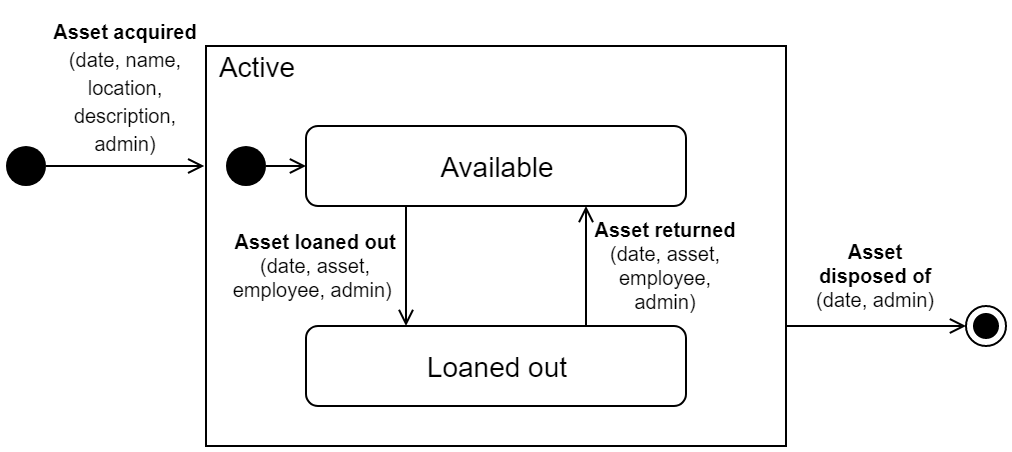
\includegraphics[width=1\textwidth]{figures/StateChart_Asset.png}
    \caption{State chart diagram for the \textbf{Asset} class}
    \label{fig:asset_statechart}
\end{figure}

An \textbf{Asset} object is created when the asset is acquired. At first, its state is \textbf{available}, and when the asset is loaned out to an employee, it changes state to \textbf{loaned out}. From any of these two states, the asset can be disposed of and no longer exist within the problem domain.
\\\\

\large{\textbf{Employee}}
\begin{figure}[H]
    \centering
    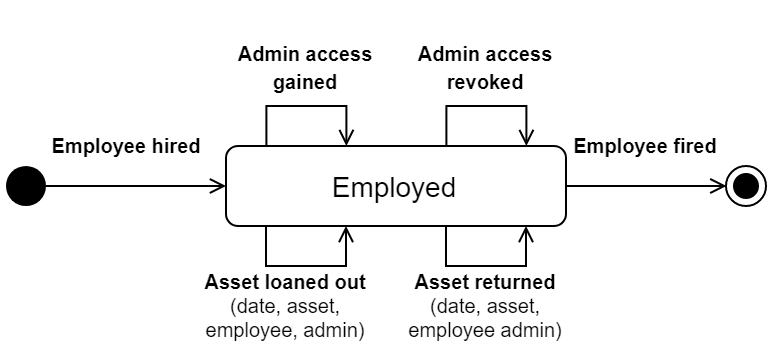
\includegraphics[width=1\textwidth]{figures/StateChart_Employee.png}
    \caption{State chart diagram for the \textbf{Employee} class}
    \label{fig:employee_statechart}
\end{figure}

An \textbf{Employee} object is created when a person is hired at the zoo and gains the status employed. An employee can potentially be granted admin access, which can later be revoked as well. An employee can also borrow an asset and return it later. The employee object seizes to exist when the person is fired.
\\\\
\todo[inline]{Combine employee and admin state charts? Or point out the sequence: admin access gained -> admin lyfe ... -> admin access revoked -> employed}


\large{\textbf{Admin}}
\begin{figure}[H]
    \centering
    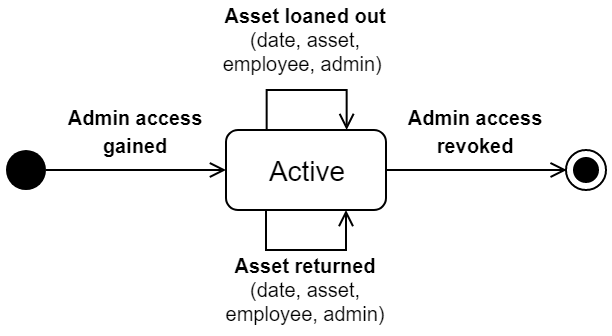
\includegraphics[width=0.8\textwidth]{figures/StateChart_Admin.png}
    \caption{State chart diagram for the \textbf{Admin} class}
    \label{fig:admin_statechart}
\end{figure}

The \textbf{Admin} object is created when an employee is granted admin access. As an admin, the employee is responsible for loaning out assets to other employees and receiving the assets when they are returned. The admin object is terminated when the employee's admin access is revoked. 
\\\\

\large{\textbf{Loan}}
\begin{figure}[H]
    \centering
    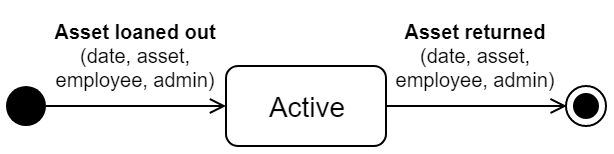
\includegraphics[width=0.8\textwidth]{figures/StateChart_Loan.png}
    \caption{State chart diagram for the \textbf{Loan} class}
    \label{fig:loan_statechart}
\end{figure}

A \textbf{Loan} object is created when an asset is loaned out and seizes to exist when the asset is returned.
\newline\par
With the behaviours of the classes described, the problem domain has been analysed. The following section will sum up the results of the analysis.